\section{Laboratory measurements and model discrepancy}\label{sec:lab}
An additional computational test uses the complex microwave measurements of the Institut Fresnel and the University of Manitoba \cite{fresnel,manitoba}. The underlying physical specimens consist of three dielectric configurations with foam and dielectric inserts at Fresnel and four dielectric objects at Manitoba. They are useful for two questions that a matched discrete simulation cannot address: how an illumination transfers to receivers outside the design arc, and how much modelling error an exclusion claim can tolerate.

For each laboratory and frequency take every unordered pair of its specimens. Use the measured response difference on one half of the common receiving aperture to select a unit-norm coherent combination of the available incident columns. Select the strongest individual column on that same half as the control. Compare their measured complex-field differences on the opposite half and exchange the halves. Fresnel has two common source directions, at $0$ and $180$ degrees. At Manitoba twelve transmitters alternate with twelve receivers around the array. Source normalization is Euclidean in the recorded coordinates. At each frequency the two halves, and the pairs that share a target, are correlated conditions. This retrospective use of the measured matrices estimates transfer across receivers. A calibrated input power Gram and an independent physical replay would be needed to convert it into a transmit-energy experiment.

At Fresnel the coherent combination gave a larger held-out difference in 17 of 18 conditions at 4, 6 and 8 GHz. With the individual empty reference the median ratio was 1.088 and the range was 0.995--1.266. Replacing those references by a common empty reference gave 1.088 and 0.993--1.266. At Manitoba, using the larger metal reference and the initial empty acquisition, the corresponding count was 45 of 84, the median was 1.021 and the range was 0.350--2.741. Calibrating with the smaller reference reduced the count to 32 of 84, with median 0.877. Figure~\ref{fig:lab} shows the full distribution. A commanding improvement on the design half can disappear on the held receivers. Calibration choice is especially important for the second apparatus.

For a nonlinear material bound the error ball must include the loaded instrument and discretization discrepancy. In a previously evaluated contrast test, the large nylon cylinder at 3 GHz left a margin of $4.018\%$ of the observed norm after reference errors were allowed for. Only a loaded discrepancy below that margin would permit exclusion of all media with contrast at most one. Fitting the empty chamber does not supply such a uniform bound. The nonnegative Born residual exceeded the empty-field reference error in 3 of 9 Fresnel and 25 of 28 Manitoba object--frequency conditions. These finite comparisons describe the scale of model error. They do not establish a measured inclusion-location or classification guarantee.
\begin{figure}[tp]\centering
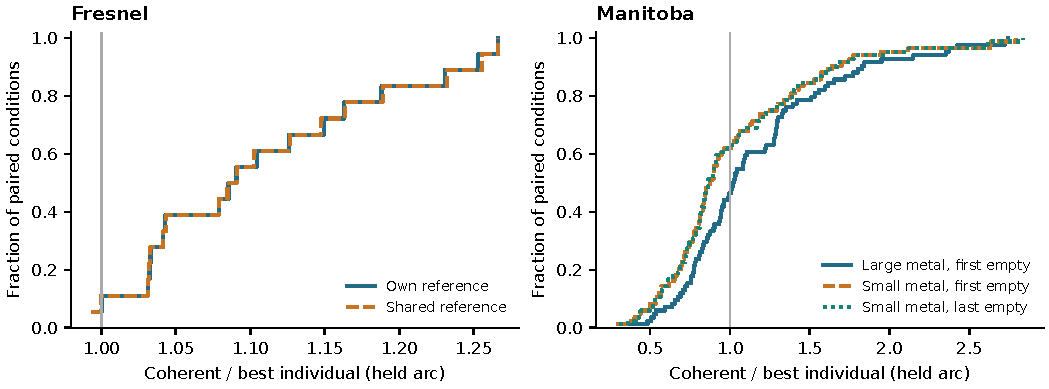
\includegraphics[width=.94\linewidth]{measured}
\caption{Held-receiver field differences for two measured specimens, normalized by the field difference of the strongest individual transmitter chosen on the design arc. The central line denotes equal performance. Each distribution counts pair, frequency and receiving-split combinations. Recalibration of the Manitoba data changes the ranking while leaving the physical specimens fixed.}\label{fig:lab}
\end{figure}
